\documentclass{article}
\usepackage[utf8]{inputenc}
\usepackage{indentfirst}
\usepackage{enumitem, amsmath, amssymb}
\usepackage[a4paper, margin=0.8in]{geometry}
\usepackage{graphicx, caption}

\graphicspath{ {./images/} }


\title{Algebraic Topology  --- Feedback Exercise 4}
\author{Samuel Jackson --- 2520998j}
\date{\today}

\begin{document}

\maketitle

\newcommand{\R}{\mathbb{R}}
\newcommand{\Z}{\mathbb{Z}}
\newcommand{\N}{\mathbb{N}}
\newcommand{\fund}{\pi_1}
\newcommand{\pind}{p_{\ast}}

%%%
\begin{center}
    \section*{Question (1)}
\end{center}

\begin{flushleft}
    For this question, we wish to apply Van Kampen's theorem so we must find open sets of $X$. We choose our sets to be $U = \{(x, y, z) \in X : x < 3\}$ and $V = \{(x,y,z) \in X : x > 0\}$. These are clearly open sets. The illustration below also helps to determine the intersection of the two sets, which is defined $U \cap V = \{(x,y,z) \in X : 0 < x < 3\}$. 

    \begin{figure}[h]
        \minipage[t]{0.32\textwidth}
            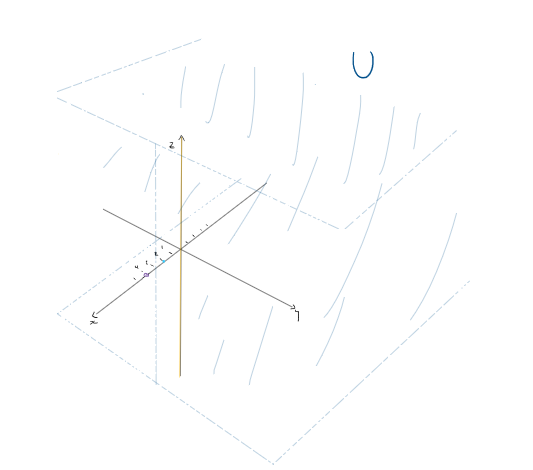
\includegraphics[height=4cm, width=\linewidth]{images/u-openset.png}
            \caption*{Illustration of open set $U$}
        \endminipage\hfill
        \minipage[t]{0.32\textwidth}
            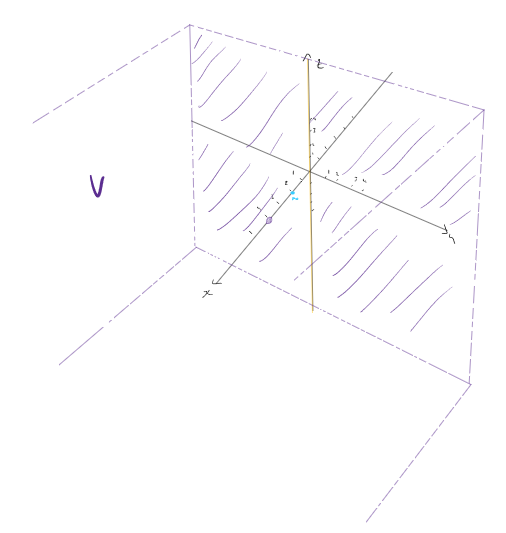
\includegraphics[height=4cm, width=\linewidth]{images/v-openset.png}
            \caption*{Illustration of open set $V$}
        \endminipage\hfill
        \minipage[t]{0.32\textwidth}
            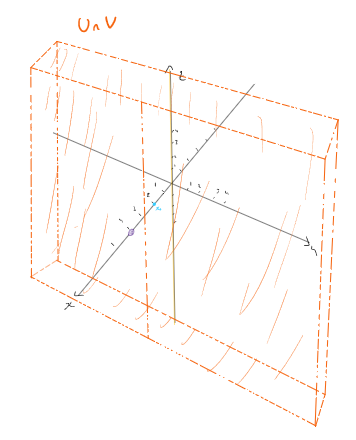
\includegraphics[height=4cm, width=\linewidth]{images/intersect-openset.png}
            \caption*{Illustration of the intersection $U \cap V$}
        \endminipage
    \end{figure}

    The open set $U \cap V$ deformation retracts to a point and, hence, is simply connected. Given $U$ and $V$ are similarly path connected, with $X = U \cup V$, then we can use the basic version of Van Kampen's theorem. First, we note that $\fund(U) \cong \Z$ and $\fund(V) \cong 1$. We use Van Kampen's and see that $\fund(X) \cong \fund(U) \ast \fund(V)$. Consequently, $\fund(X, x_0) \cong \Z$.
     
\end{flushleft}
%%%
\begin{center}
    \section*{Question (2)}
\end{center}

\begin{flushleft}
    Similar to the last question, we aim to find appropriate open sets for the given set $X$. Let $U$ be the open set which covers all of $S^2$ as well as a small open annulus around the equator, extending into the $xy$-plane. Let $V$ be the open set of the $xy$-plane as well as a small section of the sphere around the equator. Note that $x_0$ is contained in both $U$ and $V$. The illustration below should make the open sets clear, alongside their intersection. \newline 

        \begin{figure}[!h]
        \minipage[t]{0.32\textwidth}
            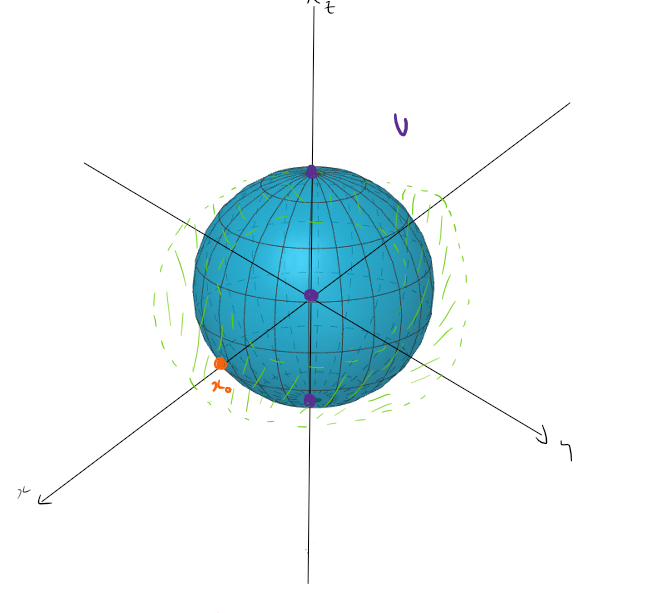
\includegraphics[height=5cm, width=\linewidth]{images/q2-u-openset.png}
            \caption*{Illustration of open set $U$}
        \endminipage\hfill
        \minipage[t]{0.32\textwidth}
            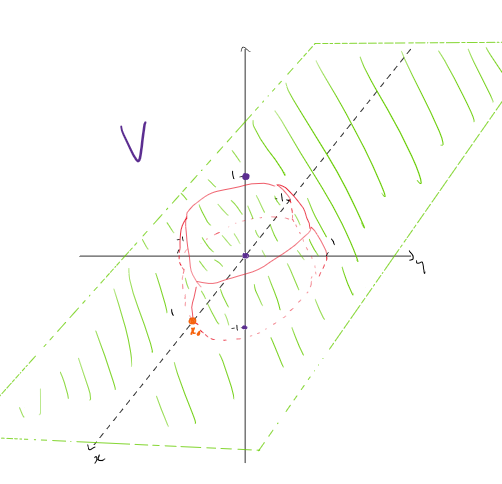
\includegraphics[height=5cm, width=\linewidth]{images/q2-v-openset.png}
            \caption*{Illustration of open set $V$}
        \endminipage\hfill
        \minipage[t]{0.32\textwidth}
            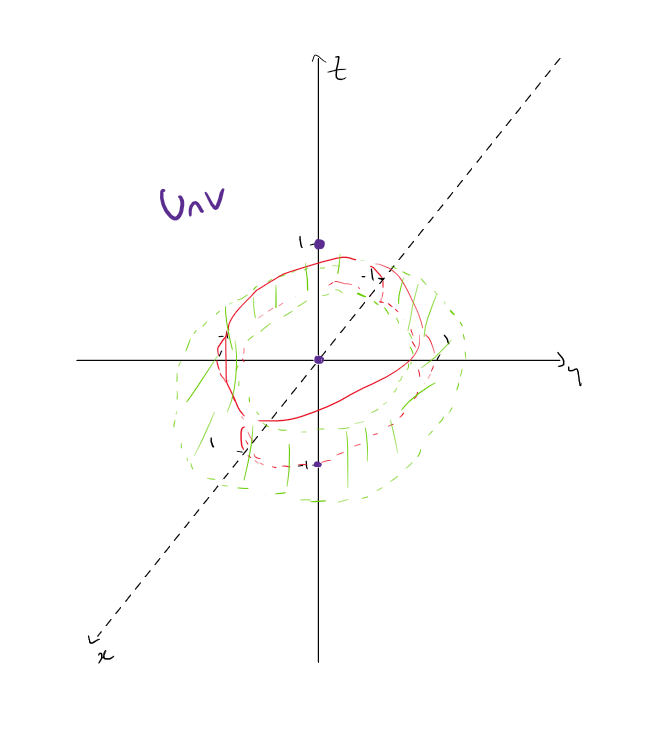
\includegraphics[height=5cm, width=\linewidth]{images/q2-intersect-openset.png}
            \caption*{Illustration of the intersection $U \cap V$}
        \endminipage
    \end{figure}

    We see that $U$ and $V$ are path-connected, open sets such that $X = U \cup V$. Furthermore, the intersection $U \cap V$ deformation retracts to an open annulus, which is path-connected. Hence, we have all the conditions to apply the full version of Van Kampen's. We first note that $\fund(U) \cong \Z \cong \langle u : - \rangle$ and $\fund(V) \cong \Z \cong \langle v : - \rangle$. Similarly, we consider $\fund(U \cap V) = \Z \cong \langle a : - \rangle$. We consider the inclusion maps $i : U \cap V \rightarrow U$ and $j : U \cap V \rightarrow V$ which create the induced homomorphisms: $i_\ast : \fund(U \cap V) \rightarrow \fund(U)$, $j_\ast : \fund(U \cap V) \rightarrow \fund(V)$ in order to apply Van Kampen's. Since there is only one generator in $\fund(U \cap V)$, we only need to add one relation to our free product of $\fund(U) \ast \fund(V)$. \newline 

    The theorem states that we need $i_\ast(a) = j_\ast(a)$, for the generator $a \in \fund(U \cap V)$. Given that $\fund(U)$ and $\fund(V)$ only have one generator and the homomorphism is induced by the inclusion map then it is defined by the generators so $i_\ast(a) = u$ and $j_\ast(a) = v$. This gives the relation that $u = v$. Hence, through Tietze transformations, $\fund(X) = \langle u, v : u = v \rangle \cong \langle u : - \rangle \cong \Z$. (Note that this question can also be entirely answered using deformation retractions on the original disjoint union).

    
\end{flushleft}
\end{document}
